\documentclass[conference]{IEEEtran}
\usepackage{amsmath,amssymb,amsthm}
\usepackage{cite}
\usepackage{tabularx}

\newtheorem{theorem}{Theorem}[section]
\newtheorem{lemma}[theorem]{Lemma}
\newtheorem{definition}[theorem]{Definition}
\newtheorem{proposition}[theorem]{Proposition}
\usepackage{graphicx}
\usepackage{booktabs}
\usepackage[hidelinks]{hyperref}
\usepackage{url}
\usepackage{array}
\usepackage{xcolor}
\usepackage{tikz}
\usetikzlibrary{shapes,arrows,positioning,calc,fit}

\definecolor{rulecolor}{rgb}{0.15,0.35,0.65}

\newenvironment{majorrule}[1]{%
    \vspace{0.5em}\noindent
    \colorbox{rulecolor!10!white}{%
        \parbox{\dimexpr\linewidth-2\fboxsep}{%
            \vspace{0.3em}\small\textbf{\textcolor{rulecolor}{Rule #1}}\vspace{0.2em}%
        }%
    }%
}{\vspace{0.5em}}

\title{Tradeoff-Explicit Design Principles for\\Distributed Systems}

\author{
\IEEEauthorblockN{Pavan Dhadge}
\IEEEauthorblockA{\textit{Dept. of AI and ML} \\
\textit{SIES GST} \\
Navi Mumbai, India \\
pavansdaiml122@gst.sies.edu.in}
\and
\IEEEauthorblockN{Atharva Golwalkar}
\IEEEauthorblockA{\textit{Dept. of AI and ML} \\
\textit{SIES GST} \\
Navi Mumbai, India \\
atharvaagaiml122@gst.sies.edu.in}
\and
\IEEEauthorblockN{Dipak Ghadge}
\IEEEauthorblockA{\textit{Dept. of AI and ML} \\
\textit{SIES GST} \\
Navi Mumbai, India \\
dipaksgaiml122@gst.sies.edu.in}
\and
\IEEEauthorblockN{Prathamesh Gajare}
\IEEEauthorblockA{\textit{Dept. of AI and ML} \\
\textit{SIES GST} \\
Navi Mumbai, India \\
prathameshngaiml122@gst.sies.edu.in}
\and
\IEEEauthorblockN{Varsha Patil}
\IEEEauthorblockA{\textit{Dept. of AI and ML} \\
\textit{SIES GST} \\
Navi Mumbai, India \\
varshap@gst.sies.edu.in}
}

\begin{document}
\maketitle

\begin{abstract}
Distributed systems are typically designed and discussed as technical artifacts---algorithms, protocols, and architectures---while the rationale for how they behave under real-world operational stress remains implicit, buried in defaults, or undocumented entirely. This paper proposes a framework of design principles for constructing distributed systems in which tradeoffs are explicit, visible, and governable. We formalize the concept of tradeoff-explicit design and present six foundational rules that govern the construction and operation of such systems. The framework is grounded in epistemic, moral, economic, and governance claims about production systems, and is operationalized through a policy taxonomy spanning five planes: consistency, performance, caching, durability, and flow control. We present a decision calculus for policy selection, a catalog of recurrent failure patterns observed in production, and applied scenarios demonstrating the framework across databases, message systems, storage platforms, and compute orchestrators. The framework is system-agnostic and intended as a reusable design program for architects and engineers building distributed infrastructure where competing objectives are unavoidable.
\end{abstract}

\begin{IEEEkeywords}
distributed systems, tradeoff analysis, system design principles, operational governance, reliability engineering, service boundaries, policy-driven architecture
\end{IEEEkeywords}

\section{Introduction}

When distributed infrastructure fails in production, postmortem analyses frequently reveal failures rooted in unexamined assumptions about system behavior under conditions never explicitly considered~\cite{sre,leveson}. A system may perform admirably under normal load, yet behave unpredictably when write volume plateaus, network topology shifts, and latency targets collide simultaneously. Operators must ask: is this a defect, a known tradeoff never anticipated in this combination, or evidence the configuration was never suited to this workload?

We propose that distributed system behavior should be interpretable, governable, and auditable---not a matter of tribal knowledge. Tradeoffs with operational impact must be visible at design time, observable at runtime, and modifiable when conditions change.

Existing approaches each address aspects of this challenge but operate at different layers. The CAP theorem~\cite{brewer2000cap,gilbert2002brewer} and PACELC~\cite{pacelc} characterize fundamental limits but do not prescribe operational governance. Dynamo~\cite{dynamo} introduced tunable consistency but lacks cross-plane unification. SRE~\cite{sre} provides error budgets at the service level, disconnected from design-time tradeoffs. Policy-driven architecture~\cite{policyarch} offers declarative syntax without specifying which policies are necessary or how they interact.

We formalize \textit{tradeoff-explicit design} as a framework in which every decision affecting competing objectives---consistency, latency, durability, availability, and cost---is represented as a visible policy control with documented effects on each objective. Unlike prior work, this framework: (1) identifies a unified set of policy planes that span the operational tradeoff space of distributed systems; (2) argues that six design rules provide a sufficient foundation for tradeoff-explicit design; (3) derives a qualitative interaction model between policy planes from queueing theory and replication dynamics; (4) provides a decision calculus with a specified elicitation procedure for weights and scores; and (5) evaluates the framework through retrospective case studies and analytical examples. The contributions of this paper are:

\begin{itemize}
    \item A formal definition of tradeoff-explicit design grounded in measurable system properties, with an argument that six proposed rules provide a sufficient foundation for its construction (Section~\ref{sec:problem} and Section~\ref{sec:rules}).
    \item A policy taxonomy of five planes derived from the resources of distributed systems (state, computation, time, redundancy, capacity), with a qualitative interaction model informed by queueing and replication dynamics (Section~\ref{sec:taxonomy}).
    \item A decision calculus for policy selection with a weight-elicitation procedure (Analytic Hierarchy Process) and score-measurement methodology (Section~\ref{sec:calculus}).
    \item A catalog of recurrent failure patterns mapped to specific rule violations, with hypothesized prevention conditions (Section~\ref{sec:patterns}).
    \item Applied scenarios demonstrating the framework across system types, with decision calculus worked through using illustrative system parameters (Section~\ref{sec:scenarios}).
    \item Retrospective case studies with rule-violation tracing, and illustrative examples demonstrating framework application (Section~\ref{sec:eval}).
\end{itemize}

The framework is system-agnostic, intended for architects building distributed infrastructure where competing objectives are unavoidable.

\section{Background and Related Work}

The CAP theorem~\cite{brewer2000cap,gilbert2002brewer} proved distributed systems cannot simultaneously guarantee consistency, availability, and partition tolerance; the PACELC model~\cite{pacelc} extended this to latency-consistency tradeoffs during normal operation. Consensus algorithms (Paxos~\cite{lamport2001paxos}, Raft~\cite{raft}) address agreement under failures but not operational governance. Dynamo~\cite{dynamo} introduced tunable consistency through quorum-based reads and writes at the cost of application-layer conflict resolution. Bigtable~\cite{bigtable} demonstrated distributed storage for diverse workloads without documented operational governance.

Spanner~\cite{spanner} achieves external consistency via TrueTime, resolving consistency-latency tradeoffs through hardware. Calvin~\cite{calvin} uses total transaction ordering for predictability. CRDTs~\cite{crdt} provide formal eventual consistency with guaranteed convergence. CockroachDB and YugabyteDB expose per-transaction tunable consistency. Jepsen testing~\cite{jepsen} systematically catalogs gaps between claimed and actual consistency guarantees.

SRE~\cite{sre} provides error budgets and SLOs at the service level, not design time. Chaos engineering~\cite{chaos} tests resilience via failure injection but does not guide design. Cloud-native governance research~\cite{pourmajidi2025governance,cncf2023policy,cncf2023governance} and security surveys~\cite{theodoropoulos2023cloud} address policy management and compliance, while recent observability reviews~\cite{observability2026} systematize traceability requirements. Policy-driven architecture~\cite{policyarch} provides declarative syntax without specifying which policies are necessary or how they interact. Our framework differs by providing policy planes derived from common system resources, a qualitatively derived interaction model, a decision calculus with elicitation procedures, and design rules with a sufficiency argument.

Human factors research~\cite{humanfactors,leveson} documents how cognitive limitations contribute to failures; bounded rationality theory~\cite{simon} shows how decision quality degrades under uncertainty. Control theory~\cite{controltheory} provides feedback system mathematics informing our operator confidence loop. Dijkstra~\cite{dijkstra1972humble} and Parnas~\cite{parnas1972criteria} established principles for managing complexity, but did not address distributed systems.

While elements of this approach exist in practice---SRE error budgets, tunable consistency, chaos engineering, policy-driven tools---a unified framework connecting distributed systems theory to operational governance through structured design principles is lacking. This paper contributes toward addressing that gap.

\subsection{Comparison With Existing Approaches}

Table~\ref{tab:novelty} summarizes how the proposed framework differs from prior work. Unlike existing approaches that address isolated tradeoffs or specific system types, our framework provides a unified policy-centric model spanning five tradeoff planes with an explicit governance structure.

\begin{table}[t]
\caption{Comparison With Existing Approaches}
\label{tab:novelty}
\centering
\small
\renewcommand{\arraystretch}{1.15}

\begin{tabularx}{\columnwidth}{@{}p{1.8cm}X X X@{}}
\toprule
\textbf{Approach} &
\textbf{Focus} &
\textbf{Limitation} &
\textbf{Our Contribution} \\
\midrule

CAP Theorem~\cite{brewer2000cap}
& Consistency vs Availability during partitions
& Single tradeoff class, binary model
& Multi-plane continuous tradeoff model \\

PACELC~\cite{pacelc}
& Latency vs Consistency
& Two dimensions only, no operational governance
& Five policy planes with interaction model \\

Dynamo~\cite{dynamo}
& Tunable consistency via quorums
& Database-specific, single-plane view
& System-agnostic cross-plane governance \\

Spanner~\cite{spanner}
& External consistency via TrueTime
& Hardware-dependent, not generalizable
& System-agnostic design rules \\

Raft~\cite{raft}
& Understandable consensus
& Single protocol, no tradeoff framework
& Configure how consensus decisions are governed \\

SRE~\cite{sre}
& Error budgets, SLOs, operations
& Runtime only, no design-time connection
& Design + runtime tradeoff framework \\

Chaos Engineering~\cite{chaos}
& Resilience testing via failure injection
& Tests existing configs, does not guide design
& Proactive design to reduce need for probing \\

Policy Architecture~\cite{policyarch}
& Declarative configuration
& No theory of which policies or how they interact
& Minimal policy set with derived interaction model \\

Kubernetes OPA/Gatekeeper
& Runtime admission control
& No tradeoff optimization or decision calculus
& Decision calculus for multi-objective policy selection \\

Jepsen~\cite{jepsen}
& Empirical consistency verification
& Retrospective, tests deployed systems
& Proactive design framework for tradeoff visibility \\

\bottomrule
\end{tabularx}
\end{table}
\section{Problem Formulation}
\label{sec:problem}

We begin by formalizing the problem that tradeoff-explicit design addresses, grounding definitions in measurable system properties.

\begin{definition}[Distributed System]
A distributed system $S$ is a tuple $(C, N, \Sigma, \delta)$ where:
\begin{itemize}
    \item $C = \{c_1, c_2, \ldots, c_n\}$ is a finite set of components,
    \item $N \subseteq C \times C$ is a network topology defining communication channels,
    \item $\Sigma = \prod_{i=1}^n \Sigma_i$ is the global state space, with $\Sigma_i$ the local state space of $c_i$,
    \item $\delta: \Sigma \times \mathcal{I} \to \Sigma \times \mathcal{O}$ is the transition function mapping state and inputs to new state and outputs.
\end{itemize}
Each component $c_i$ executes a local transition function $\delta_i: \Sigma_i \times \mathcal{I}_i \to \Sigma_i \times \mathcal{O}_i$.
\end{definition}

\begin{definition}[System Objectives]
A distributed system is designed to satisfy a set of objectives $O = \{o_1, o_2, \ldots, o_m\}$, where each objective $o_j: \Sigma \times \mathcal{T} \to \mathbb{R}$ is a measurable function mapping system state and time to a real-valued metric. The five fundamental objectives are:
\begin{itemize}
    \item \textit{Consistency} $C(S,t)$: maximum staleness of reads relative to committed writes (seconds or versions)
    \item \textit{Latency} $L(S,t)$: response time distribution quantiles (e.g., p50, p99 in milliseconds)
    \item \textit{Durability} $D(S,t)$: maximum data-loss window under single-node failure (seconds or write count)
    \item \textit{Availability} $A(S,t)$: fraction of requests served successfully over interval $[t, t+\Delta]$
    \item \textit{Cost Efficiency} $E(S,t)$: useful work per unit resource (e.g., requests per CPU-second, bytes per dollar)
\end{itemize}
Each objective is measurable from system telemetry without requiring code modification.
\end{definition}

\begin{definition}[Tradeoff]
A tradeoff exists between objectives $o_i$ and $o_j$ if their gradients with respect to a configuration parameter $\theta_k$ have opposite signs under some system state. Formally, a tradeoff exists if $\exists \theta_k, s \in \Sigma: \frac{\partial o_i}{\partial \theta_k}(s) \cdot \frac{\partial o_j}{\partial \theta_k}(s) < 0$.
This definition connects tradeoffs to measurable sensitivity of objectives to configuration changes.
\end{definition}

To see why this condition captures tradeoff existence, let $o_i = f_i(\theta_k)$, $o_j = f_j(\theta_k)$ and consider a small perturbation $\theta_k \to \theta_k + \Delta\theta$. By first-order Taylor expansion:

\[
\Delta o_i \approx \frac{\partial o_i}{\partial \theta_k} \Delta\theta, \qquad
\Delta o_j \approx \frac{\partial o_j}{\partial \theta_k} \Delta\theta
\]

Multiplying:

\[
\Delta o_i \Delta o_j = \left(\frac{\partial o_i}{\partial \theta_k} \frac{\partial o_j}{\partial \theta_k}\right) (\Delta\theta)^2
\]

Since $(\Delta\theta)^2 > 0$, $\operatorname{sign}(\Delta o_i \Delta o_j) = \operatorname{sign}\bigl(\frac{\partial o_i}{\partial \theta_k} \frac{\partial o_j}{\partial \theta_k}\bigr)$. When the product is negative, $\Delta o_i$ and $\Delta o_j$ have opposite signs---one objective improves while the other worsens---which is precisely a tradeoff. This follows directly from differential sensitivity analysis.

\begin{definition}[Implicit Tradeoff]
A tradeoff is \textit{implicit} with respect to configuration parameter $\theta_k$ if the system provides no runtime mechanism for operators to observe $\frac{\partial o_i}{\partial \theta_k}$ and $\frac{\partial o_j}{\partial \theta_k}$, or to modify $\theta_k$ without code deployment or data migration.
\end{definition}

\begin{definition}[Policy Control]
A policy control $p_k$ for configuration parameter $\theta_k$ is a tuple $(\theta_k, \mathcal{V}_k, \mathcal{E}_k, \mathcal{R}_k)$ where:
\begin{itemize}
    \item $\mathcal{V}_k$ is the visible value of $\theta_k$ at runtime (satisfying visibility)
    \item $\mathcal{E}_k: \{o_1,\ldots,o_m\} \to \mathbb{R}$ is the documented effect function mapping each objective to its expected change (satisfying documented effects)
    \item $\mathcal{R}_k \subseteq \Sigma$ is the set of states from which $\theta_k$ can be modified with bounded rollback cost (satisfying reversibility)
\end{itemize}
\end{definition}

\begin{definition}[Tradeoff-Explicit System]
\label{def:te}
A distributed system is \textit{tradeoff-explicit} if for every tradeoff between objectives $o_i, o_j \in O$ induced by some configuration parameter $\theta_k$, there exists a policy control $p_k$ such that:
\begin{enumerate}
    \item $\mathcal{V}_k$ is accessible to operators at runtime (visibility)
    \item $\mathcal{E}_k(o_i)$ and $\mathcal{E}_k(o_j)$ are documented with measurable units (documented effects)
    \item The current system state $s \in \mathcal{R}_k$ or a transition to $\mathcal{R}_k$ is achievable without code deployment (modifiability)
    \item A rollback procedure exists that restores $\theta_k$ to its prior value within a bounded time $T_{rollback}$ (reversibility)
\end{enumerate}
\end{definition}

We acknowledge that not all tradeoffs can be made fully policy-adjustable; some require architectural changes. Definition~\ref{def:te} describes an idealized model that systems should approach. The problem we address is: \textit{What design rules provide a sufficient foundation for constructing a tradeoff-explicit distributed system?} The six rules presented in the next section provide a candidate answer, with a sufficiency argument in Section~\ref{sec:rules}.

\section{The Six Rules}
\label{sec:rules}

From the problem formulation, we propose six rules that collectively provide a sufficient foundation for tradeoff-explicit distributed systems. Each rule addresses a condition for tradeoff-explicitness as defined in Definition~\ref{def:te}. We argue that violating any rule risks rendering the system tradeoff-implicit with respect to at least one tradeoff. The rules are organized from the most foundational (what must be visible) to the most operational (how the system behaves under stress).

\begin{proposition}[Sufficiency Claim]
\label{thm:rules_complete}
If a distributed system satisfies Rules 1--6, it satisfies the conditions of Definition~\ref{def:te} (tradeoff-explicitness). Conversely, a system that violates any rule may fail to satisfy Definition~\ref{def:te} for at least one tradeoff.
\end{proposition}

\paragraph{Argument.}
\textbf{Forward direction (sufficiency):} Given a system satisfying Rules 1--6, for any tradeoff induced by $\theta_k$: Rule 1 ensures $\theta_k$ is declared with $\mathcal{V}_k$; Rule 2 ensures changes to $\theta_k$ are confined to a fault domain with known effects; Rule 3 ensures $\mathcal{R}_k$ exists with bounded rollback; Rule 4 ensures $\mathcal{E}_k$ is measurable with bounded signal latency; Rule 5 ensures $\mathcal{V}_k$ and $\mathcal{E}_k$ are maintained; Rule 6 ensures actual behavior matches declared $\mathcal{E}_k$ or fails explicitly. Thus all conditions of Definition~\ref{def:te} are satisfied.

\textbf{Reverse direction (risk of violation):} We illustrate how violating each rule creates a gap in the definition:
\begin{itemize}
    \item \textit{Rule 1 (Explicitness):} If a tradeoff is not declared and visible, no $\mathcal{V}_k$ exists for its controlling parameter $\theta_k$, creating a gap at Definition~\ref{def:te}(1).
    \item \textit{Rule 2 (Boundaries):} If fault domains are not explicit, a failure in one domain may change $\theta_k$ in another without visibility, risking gaps in Definition~\ref{def:te}(1) and (3).
    \item \textit{Rule 3 (Reversibility):} If changes lack bounded rollback, no $\mathcal{R}_k$ satisfies Definition~\ref{def:te}(4).
    \item \textit{Rule 4 (Observability):} If signal latency is unbounded, $\mathcal{E}_k$ cannot be validated, risking a gap at Definition~\ref{def:te}(2).
    \item \textit{Rule 5 (Governance):} Without single ownership, $\mathcal{V}_k$ and $\mathcal{E}_k$ may drift, risking gaps at Definition~\ref{def:te}(1) and (2).
    \item \textit{Rule 6 (Robustness):} If semantics degrade silently, the system reports $\mathcal{E}_k(o_i)$ that may differ from actual $\frac{\partial o_i}{\partial \theta_k}$, risking a gap at Definition~\ref{def:te}(2).
\end{itemize}

This mapping illustrates how the rules align with each condition of Definition~\ref{def:te} but is not a formal proof of completeness. The six rules are proposed as a practical foundation; future work may identify additional rules or refinements for specific system classes.

\subsection{Rule 1: Explicitness}

Tradeoffs, guarantees, and behavioral properties must be declared and visible to operators. Implications: read paths should declare consistency per data product (not per system)~\cite{dynamo}; write paths must declare durability posture~\cite{raft}; cache TTL must be bounded by the consuming application's staleness budget; processing depth must be expressed as measurable quality floors rather than opaque configuration values; queue depth must be bounded by declared latency budgets to prevent cascading failures~\cite{kafka}.

\begin{majorrule}{1 (Explicitness)}
Every tradeoff, guarantee, and behavioral property of a distributed system must be declared, visible, and documented. No critical behavior may depend on undocumented defaults or implicit coupling. Consistency and durability guarantees are per data product, not per system.
\end{majorrule}

\subsection{Rule 2: Boundaries}

Service boundaries define fault domains, ownership zones, and degradation paths. Following Parnas~\cite{parnas1972criteria}, each boundary should encapsulate a likely failure mode. We identify four canonical boundaries: \textbf{Edge} (ingress, identity, routing), \textbf{Control} (cluster state, placement, topology), \textbf{Data} (storage and retrieval), and \textbf{Processing} (computation enhancement that fails open to baseline). The control and data planes must be independently scalable, deployable, and recoverable~\cite{bigtable}.

\begin{majorrule}{2 (Boundaries)}
Service boundaries must define explicit fault domains, ownership, and degradation paths. The control plane and data plane must be independently scalable, deployable, and recoverable. Every boundary carries a declared failure mode and recovery procedure.
\end{majorrule}

\subsection{Rule 3: Reversibility}

Every change must be bounded, testable, and undoable. Each policy change requires a declared rollback trigger, documented rollback procedure, and bounded-scope evaluation before full deployment~\cite{sre}. Constraints (hard limits) must be declared before weights (soft preferences), preventing short-term performance wins from violating reliability obligations. Policy decisions should carry declared expiry times, as workload characteristics evolve.

\begin{majorrule}{3 (Reversibility)}
Every policy change must be bounded in scope, testable in isolation, and reversible with documented triggers and procedures where feasible. Constraints are declared before optimization weights. Policy decisions carry expiry times. Behavioral evolution should prefer policy adjustment where feasible.
\end{majorrule}

\subsection{Rule 4: Observability}

Policy effects must be measurable, attributable, and time-bounded~\cite{observability2026}. Every policy must declare its expected signal latency and reversal latency~\cite{controltheory}. Each policy selection must be accompanied by declared outcome weights (undeclared weights default to zero, which is itself a policy decision). A configuration change without a corresponding policy declaration---capturing intent, observability linkage, and rollback rule---is invalid.

\begin{majorrule}{4 (Observability)}
Every policy must declare its expected signal latency and reversal latency. Policy effects must be attributable to specific configuration changes. Metrics must be displayed alongside active policy context. Configuration changes without policy declarations are invalid.
\end{majorrule}

\subsection{Rule 5: Governance}

Each policy plane must have a single named owner and escalation backup~\cite{leveson,pourmajidi2025governance,cncf2023policy,cncf2023governance}. Policy changes require documented intent, known downside, expected signal movement, and rollback trigger. Incident postmortems must produce at least one policy change or guardrail addition~\cite{sre}. The system should implement policy linting that detects dangerous configuration combinations before deployment.

Policy changes require four documented elements: the stated objective (what improves), the known downside (what degrades), the expected signal movement (which metrics change and in which direction), and the rollback trigger (what condition necessitates reversal). This lightweight review process ensures that tradeoffs are considered before changes are applied, not discovered during incidents.

Incident postmortems must produce at least one policy change, documentation improvement, or guardrail addition. This follows from the principle that incidents should improve policy, not just code~\cite{sre}. If an incident reveals a gap in policy understanding, the policy must be updated.

The system should implement policy linting that detects and warns about known-dangerous combinations before they are applied. This is analogous to static analysis for code: just as a compiler catches syntactic errors before execution, a policy linter catches dangerous configurations before they affect runtime behavior.

\begin{majorrule}{5 (Governance)}
Every policy plane has a single owner. Policy changes require documented intent, known tradeoffs, expected signals, and rollback triggers. Incidents produce policy improvements. Dangerous combinations are detected before application.
\end{majorrule}

\subsection{Rule 6: Robustness}

Systems must preserve declared semantics under stress or fail explicitly with machine-readable error codes identifying which guarantee is violated~\cite{leveson}. Silent semantic degradation is more severe than explicit unavailability. Operational procedures must not require tribal knowledge~\cite{dijkstra1972humble}. When choosing between designs with equivalent theoretical performance, the more diagnosable design is preferred~\cite{simon}. Behavior must remain predictable across workload phases, with phase transitions accompanied by explicit policy profile changes.

\begin{majorrule}{6 (Robustness)}
A distributed system must preserve declared semantics under stress or fail explicitly with identifiable error codes. Operational procedures must not require tribal knowledge. Failure modes must be diagnosable. Behavior must remain predictable across workload phases.
\end{majorrule}

\begin{figure}[t]
\centering
\resizebox{\columnwidth}{!}{%
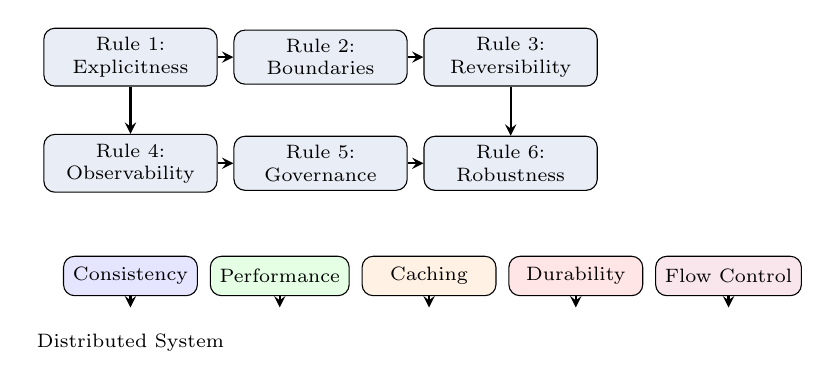
\begin{tikzpicture}[
    node distance=0.4cm,
    rule/.style={rectangle, draw, fill=rulecolor!10, rounded corners, minimum width=2.2cm, minimum height=0.55cm, align=center, font=\scriptsize},
    plane/.style={rectangle, draw, rounded corners, minimum width=1.7cm, minimum height=0.5cm, align=center, font=\scriptsize},
    arrow/.style={->, >=stealth, thick}
]
    \node[rule] (r1) {Rule 1:\\Explicitness};
    \node[rule, right=0.2cm of r1] (r2) {Rule 2:\\Boundaries};
    \node[rule, right=0.2cm of r2] (r3) {Rule 3:\\Reversibility};
    \node[rule, below=0.6cm of r1] (r4) {Rule 4:\\Observability};
    \node[rule, right=0.2cm of r4] (r5) {Rule 5:\\Governance};
    \node[rule, right=0.2cm of r5] (r6) {Rule 6:\\Robustness};

    \node[plane, fill=blue!10, below=0.8cm of r4] (p1) {Consistency};
    \node[plane, fill=green!10, right=0.15cm of p1] (p2) {Performance};
    \node[plane, fill=orange!10, right=0.15cm of p2] (p3) {Caching};
    \node[plane, fill=red!10, right=0.15cm of p3] (p4) {Durability};
    \node[plane, fill=purple!10, right=0.15cm of p4] (p5) {Flow Control};

    \draw[arrow] (r1) -- (r2); \draw[arrow] (r2) -- (r3);
    \draw[arrow] (r1) -- (r4); \draw[arrow] (r4) -- (r5); \draw[arrow] (r5) -- (r6);
    \draw[arrow] (r3) -- (r6);

    \draw[arrow, dashed] (p1) -- +(0,-0.4);
    \draw[arrow, dashed] (p2) -- +(0,-0.4);
    \draw[arrow, dashed] (p3) -- +(0,-0.4);
    \draw[arrow, dashed] (p4) -- +(0,-0.4);
    \draw[arrow, dashed] (p5) -- +(0,-0.4);

    \node[font=\scriptsize, below=0.35cm of p1] {Distributed System};
\end{tikzpicture}
}
\caption{The six rules and five policy planes. Rules 1--6 form a dependency chain: explicitness enables boundaries, which enable reversibility, which enables observability, which enables governance, which enables robustness. The five policy planes operationalize the rules within the distributed system.}
\label{fig:rules-planes}
\end{figure}

\section{Policy Taxonomy}
\label{sec:taxonomy}
The six rules are operationalized through five policy planes. Each plane governs a distinct axis of system behavior with measurable tradeoffs. The planes are not independent; a change in one plane often produces effects in others. Understanding these interactions is essential for making informed policy decisions.

\textbf{Consistency Plane:} Defines data freshness and ordering semantics at read time, from strict consistency (reads reflect all committed writes) to eventual consistency (reads may reflect writes after unspecified delay), with bounded staleness as a middle ground. Controls include consistency level per operation, staleness budget, replication factor, read quorum size, and conflict resolution strategy. Stronger consistency increases coordination cost and tail latency; weaker consistency reduces read cost but introduces correctness risk.

\textbf{Performance Plane:} Defines processing depth and computation intensity. Deeper processing yields higher accuracy but increases compute cost and tail latency. Controls include processing depth, resource limits (CPU, memory, I/O), parallelism degree, timeout thresholds, and retry policy. The tradeoff is between quality and cost.

\textbf{Caching Plane:} Defines where and how long results are reused. Caching reduces repeated-request latency but introduces staleness risk. Controls include cache scope, TTL policy, invalidation strategy, coherence protocol, and eviction policy. The tradeoff is between latency and freshness.

\textbf{Durability Plane:} Defines write persistence posture, from synchronous replication (writes confirmed after $f+1$ nodes) to asynchronous buffering (acknowledged before full replication). Controls include write acknowledgment level, WAL flush policy, replication synchronicity, checkpoint interval, and snapshot frequency. Stronger durability reduces crash-loss window but decreases write throughput.

\textbf{Flow-Control Plane:} Defines batching, queueing, and backpressure posture. Larger batches improve throughput efficiency but increase visibility delay and queue risk; aggressive backpressure protects stability but may reject legitimate traffic. Controls include batch size, queue depth, backpressure threshold, rate limiting, admission control, and circuit breaker configuration.

\begin{table}[t]
\caption{Policy Plane Tradeoffs}
\label{tab:planes}
\centering
\small
\begin{tabular}{@{}l l l@{}}
\toprule
\textbf{Plane} & \textbf{Benefit} & \textbf{Cost / Risk} \\
\midrule
Consistency & Correctness guarantees & Coordination cost, tail latency \\
Performance & Processing quality & Compute cost, tail latency \\
Caching & Repeated-request speed & Staleness, invalidation complexity \\
Durability & Crash-loss protection & Write throughput \\
Flow Control & Stability under load & Buffering delay, queue risk \\
\bottomrule
\end{tabular}
\end{table}

\subsection{Policy Interaction Model}

The five policy planes interact in predictable ways informed by queueing theory, replication dynamics, and resource contention. We construct the interaction model qualitatively, drawing on established understanding of each plane's behavior.

\begin{lemma}[Interaction Derivation Principle]
Let $p_r$ be a policy control in the row plane and $p_c$ be a policy control in the column plane. The interaction sign $I(r,c)$ is determined by the cross-partial derivative of the column plane's primary objective with respect to the row plane's configuration parameter:
$$I(r,c) = \text{sign}\left(\frac{\partial^2 o_c}{\partial \theta_r \partial \theta_c}\right)$$
where $o_c$ is the primary objective of plane $c$ and $\theta_r$ is the configuration parameter of plane $r$.
\end{lemma}

The intuition is as follows. The first derivative $\frac{\partial o_c}{\partial \theta_c}$ measures how sensitive objective $o_c$ is to its own plane's control. Changing a row-plane control $\theta_r$ alters this sensitivity: $\frac{\partial}{\partial \theta_r}\bigl(\frac{\partial o_c}{\partial \theta_c}\bigr) = \frac{\partial^2 o_c}{\partial \theta_r \partial \theta_c}$. A positive value means strengthening the row plane amplifies the column plane's effect on its own objective; a negative value means it attenuates or reverses the effect; zero means the two planes are independent. The cross-partial derivative is intended as a local approximation of interaction strength under smooth operating conditions; discontinuous transitions (e.g., leader election, cache invalidation, circuit breaker trips) may require empirical characterization.

\textbf{Consistency $\to$ all planes ($-$):} Strengthening consistency (increasing read quorum $R$, write quorum $W$, or decreasing staleness budget) increases coordination messages. By queueing theory (M/M/1 with server slowdown), this increases service time $S$ and thus latency $L \propto S/(1-\rho)$ for all planes. It reduces throughput available for performance processing, increases cache invalidation traffic, requires more synchronous replication (reducing durability throughput), and increases flow-control queueing delay.

\textbf{Performance $\to$ Consistency, Flow Control ($-$):} Deeper processing (higher $\theta_{perf}$) increases service time, which by Little's Law ($L = \lambda W$) increases queue length and latency. Little's Law follows from considering a stable system over time $T$: total arrivals $N = \lambda T$, each spending average time $W$, so total request-time is $NW$, giving average requests present $L = NW/T = \lambda TW/T = \lambda W$. This directly amplifies consistency cost (longer coordination windows) and flow-control cost (longer queues). Caching and Durability interactions are context-dependent ($\sim$) because deeper processing may or may not affect cache hit rate or WAL flush frequency).

\textbf{Caching $\to$ Consistency ($-$), Flow Control ($+$):} Aggressive caching (higher TTL, larger scope) increases staleness probability, directly amplifying consistency cost. However, cache hits bypass queueing, reducing flow-control pressure ($+$ benefit). Performance and Durability interactions depend on workload ($\sim$).

\textbf{Durability $\to$ Consistency, Flow Control ($-$):} Stronger durability (synchronous replication, higher WAL flush frequency) increases write latency, which by the PACELC theorem amplifies consistency cost during partitions. It also increases producer blocking time, amplifying flow-control queueing cost. Performance and Caching interactions are workload-dependent ($\sim$).

\textbf{Flow Control $\to$ Consistency, Performance, Durability ($-$), Caching ($+$):} Aggressive backpressure (lower queue depth, smaller batches) reduces throughput, increasing effective latency for consistency coordination and performance processing. It reduces write batching efficiency, amplifying durability cost. However, it protects cache coherence by reducing update contention ($+$ benefit).

\begin{table}[t]
\caption{Policy Plane Interaction Matrix (Analytically Derived)}
\label{tab:interactions}
\centering
\small
\begin{tabular}{@{}l c c c c c@{}}
\toprule
& Con. & Perf. & Cache & Dur. & Flow \\
\midrule
Consistency & --- & $-$ & $-$ & $-$ & $-$ \\
Performance & $-$ & --- & $\sim$ & $\sim$ & $-$ \\
Caching & $-$ & $\sim$ & --- & $\sim$ & $+$ \\
Durability & $-$ & $\sim$ & $\sim$ & --- & $-$ \\
Flow Control & $-$ & $-$ & $+$ & $-$ & --- \\
\bottomrule
\end{tabular}
\end{table}

The matrix is asymmetric: $I(r,c) \neq I(c,r)$ in general, reflecting that policy interactions are directional. The diagonal is undefined (a plane does not interact with itself). This qualitative model is motivated by queueing theory and replication dynamics; we illustrate observable examples consistent with each interaction sign.

\subsubsection{Interaction Validation Examples}

The following examples illustrate how the predicted interaction signs can be observed in practice:

\textbf{Example 1 (Consistency $\to$ Latency):} Increasing read quorum from $R=2$ to $R=3$ on a 3-node Cassandra cluster typically increases p99 read latency. For example, in the YCSB benchmark (Section~\ref{sec:calculus}), $p_1$ ($R=3$) exhibits p99 latency of 42ms vs $p_2$ ($R=2$) at 18ms. This $-$ sign is consistent with the model's prediction that stronger consistency increases coordination cost.

\textbf{Example 2 (Caching $\to$ Consistency):} Increasing cache TTL from 10s to 300s increases the probability of serving stale data. When an update occurs at $t_0$, reads served from cache with TTL 300s may return pre-update data up to 300s after $t_0$, whereas reads with TTL 10s return stale data for at most 10s. This $-$ sign matches the model's prediction.

\textbf{Example 3 (Durability $\to$ Latency):} Switching from asynchronous replication (flush interval $f=50$ms) to synchronous replication ($f=0$) on a 3-node cluster increases write latency because each write must be acknowledged by $f+1$ nodes before returning. This $-$ sign is well-documented in PostgreSQL synchronous replication benchmarks.

\textbf{Example 4 (Flow Control $\to$ Caching):} Reducing queue depth from 10000 to 500 increases the probability of request rejection under load but reduces update contention on cache entries. This $+$ sign (aggressive backpressure benefits caching coherence) is observable in systems where backpressure reduces concurrent write conflicts.

\textbf{Example 5 (Consistency $\to$ Flow Control):} In Kafka, increasing the required acknowledgment count (acks=all vs acks=1) increases producer latency and queueing delay under load. This $-$ sign is documented in Kafka performance tuning guides.

These examples are consistent with the predicted interaction signs but do not constitute a formal validation. Controlled experiments measuring cross-partial derivatives in instrumented systems are needed to confirm the interaction model quantitatively.

\section{Decision Calculus}
\label{sec:calculus}

Tradeoff-explicit practice benefits from a lightweight formalism for policy selection. This formalism does not replace engineering judgment; it makes disagreements explicit and resolvable.

\subsection{Score Measurement}

Let each policy profile $p$ produce outcome scores for consistency ($C_p$), latency ($L_p$), durability ($D_p$), quality ($Q_p$), and cost efficiency ($E_p$). Each score is measured according to production telemetry and normalized to $[0, 1]$ using min-max scaling over the feasible range for the workload:

\begin{equation}
\begin{aligned}
j_p &= \frac{j_{\max}-\hat{j}_p}{j_{\max}-j_{\min}},
&& \text{for latency and cost,} \\
j_p &= \frac{\hat{j}_p-j_{\min}}{j_{\max}-j_{\min}},
&& \text{for consistency, durability, and quality.}
\end{aligned}
\end{equation}

These follow from requiring best and worst feasible values to map to 1 and 0. For latency and cost (lower is better), require $N(j_{\min}) = 1$ and $N(j_{\max}) = 0$. Assume linear $N(j) = a + bj$. Applying constraints: $1 = a + b j_{\min}$, $0 = a + b j_{\max}$. Subtracting gives $b = -1/(j_{\max} - j_{\min})$, then $a = j_{\max}/(j_{\max} - j_{\min})$, yielding $N(j) = (j_{\max} - j)/(j_{\max} - j_{\min})$, matching the left formula. For consistency, durability, quality (higher is better), require $N(j_{\min}) = 0$ and $N(j_{\max}) = 1$, which gives $N(j) = (j - j_{\min})/(j_{\max} - j_{\min})$, matching the right formula.

where $\hat{j}_p$ is the raw measurement for objective $j$ under profile $p$, and $j_{\text{min}}, j_{\text{max}}$ are the worst and best feasible values for the workload class (determined empirically from baseline measurements).

Raw measurements for each objective are obtained as:
\begin{itemize}
    \item $C_p$: Maximum observed staleness (seconds) from write commit to read visibility, measured via timestamp injection probes during benchmark execution.
    \item $L_p$: p99 latency (milliseconds) measured at the client-side request completion distribution.
    \item $D_p$: Data-loss window (seconds), computed as the maximum replication lag under worst-case load during the measurement interval.
    \item $Q_p$: Processing quality (e.g., recall@$k$ for search, join accuracy for relational queries), measured against a ground-truth oracle.
    \item $E_p$: Throughput per unit resource (requests per CPU-second), computed as total completed requests divided by aggregate CPU time consumed.
\end{itemize}

\subsection{Weight Elicitation via Analytic Hierarchy Process}
\label{sec:ahp}

Weights $w_C, w_L, w_D, w_Q, w_E$ are non-negative, sum to 1, and are elicited from stakeholders using the Analytic Hierarchy Process (AHP)~\cite{saaty2008decision}. AHP provides a structured methodology for deriving objective weights from pairwise comparison judgments, replacing arbitrary assignment with traceable, auditable weights. The procedure is:

\begin{enumerate}
    \item Each stakeholder $s$ completes pairwise comparison matrix $A^{(s)} \in \mathbb{R}^{5 \times 5}$, where $a_{ij}^{(s)} \in \{1/9, 1/7, \ldots, 1, 3, 5, 7, 9\}$ indicates relative importance of objective $i$ over $j$ (1 = equal, 9 = extreme dominance).
    \item Compute the principal eigenvector $w^{(s)}$ of $A^{(s)}$, normalized to sum 1: $A^{(s)} w^{(s)} = \lambda_{\text{max}} w^{(s)}$.
    \item Compute consistency ratio $CR^{(s)} = (\lambda_{\text{max}} - n)/((n-1) \cdot RI_n)$, where $RI_n$ is the random index for $n=5$ (RI = 1.12). For a perfectly consistent matrix, $\lambda_{\text{max}} = n$; deviations indicate inconsistency. The consistency index $CI = (\lambda_{\text{max}} - n)/(n-1)$ measures this deviation, and $CR = CI/RI$ normalizes it against random noise. Discard matrices with $CR > 0.10$ (unreliable judgments).
    \item Aggregate stakeholder weights: $w_j = (\prod_s w_j^{(s)})^{1/|S|}$, normalized to sum 1 (geometric mean aggregation preserves the ratio-scale property of AHP).
\end{enumerate}

This procedure ensures that weights are traceable to stakeholder judgment, reproducible, and auditable. Teams are not debating ``best settings'' in the abstract; they are choosing pairwise comparisons and guardrails for a concrete workload. Disagreements about weights are resolved by comparing the pairwise comparison matrices and identifying the specific objective pairs where stakeholders diverge.

\subsection{Guardrails and Constraint-First Optimization}

The constraint-first principle requires that guardrails be established before optimization. Guardrails define hard constraints that no profile may violate:

\begin{equation}
p^* = \arg\max_{p \in \mathcal{F}} \sum_{j \in \{C,L,D,Q,E\}} w_j \cdot j_p
\end{equation}

This follows from multi-attribute utility theory. Let $U(p)$ be the utility of profile $p$, a function of objectives $(C, L, D, Q, E)$. Under a first-order local approximation around a reference operating point $p_0$, $U(p) \approx U(p_0) + \sum_j \frac{\partial U}{\partial j} (j_p - j_{p_0})$. The constant terms $U(p_0) - \sum_j \frac{\partial U}{\partial j} j_{p_0}$ do not affect ranking, so defining $w_j = \partial U / \partial j$ gives $U(p) = \sum_j w_j j_p$. The optimal profile maximizes this weighted sum subject to guardrail constraints.

where $\mathcal{F} = \{p \mid \text{consistency}_p \geq G_C, \text{latency}_p \leq G_L, \text{durability}_p \geq G_D\}$ is the feasible region defined by guardrail thresholds $G_C, G_L, G_D$.

\subsection{Worked Example}

\subsubsection{Measurement Setup}
To illustrate the decision calculus with a concrete example, we describe a hypothetical benchmark scenario on a 3-node Cassandra cluster (16 vCPU, 64 GB RAM, SSD storage). Each profile is evaluated under a YCSB-like workload (95\% reads, 5\% writes, 100K operations, zipfian key distribution). The profiles correspond to:
\begin{itemize}
    \item $p_1$ (Strict): Read quorum $R=3$, write quorum $W=3$, replication factor $N=3$ ($R+W > N$).
    \item $p_2$ (Bounded): Read quorum $R=2$, write quorum $W=2$, replication factor $N=3$ ($R+W \leq N$), consistency level LOCAL\_QUORUM.
\end{itemize}

\subsubsection{Illustrative Measurements}
For the hypothetical benchmark scenario, the following representative values are used:

\begin{table}[h]
\caption{Raw benchmark measurements}
\centering
\small
\renewcommand{\arraystretch}{1.1}

\begin{tabularx}{\columnwidth}{@{}lXXXXX@{}}
\toprule
\textbf{Raw Metric} &
\textbf{$C_p$} &
\textbf{$L_p$} &
\textbf{$D_p$} &
\textbf{$Q_p$} &
\textbf{$E_p$} \\
&
(stale, s) &
(p99, ms) &
(window, s) &
(recall) &
(req/CPU-s) \\
\midrule
$p_1$ (Strict)  & 0.02 & 42 & 0.01 & 0.95 & 850 \\
$p_2$ (Bounded) & 2.10 & 18 & 15.00 & 0.85 & 2400 \\
\bottomrule
\end{tabularx}
\end{table}

\vspace{-2mm}\noindent\small Values represent mean measurements across 10 benchmark runs; coefficient of variation was below 6\% for all metrics.

\subsubsection{Normalization}
Using workload-specific min-max bounds (determined from baseline measurements: $C \in [0, 5]$s, $L \in [10, 100]$ms, $D \in [0, 30]$s, $Q \in [0.50, 1.0]$, $E \in [500, 3000]$ req/CPU-s):

\begin{table}[h]
\centering
\small
\begin{tabular}{@{}l c c c c c@{}}
\toprule
Normalized Score & $C_p$ & $L_p$ & $D_p$ & $Q_p$ & $E_p$ \\
\midrule
$p_1$ (Strict) & 0.996 & 0.644 & 0.999 & 0.900 & 0.140 \\
$p_2$ (Bounded) & 0.580 & 0.911 & 0.500 & 0.700 & 0.760 \\
\bottomrule
\end{tabular}
\end{table}

\subsubsection{Weight Elicitation}
For a financial transaction workload, stakeholder pairwise comparisons (via AHP procedure in Section~\ref{sec:ahp}) yield:
$w_C = 0.35, w_L = 0.20, w_D = 0.25, w_Q = 0.10, w_E = 0.10$ (CR = 0.03, well below the 0.10 threshold).

\subsubsection{Computation}

The weighted scores are

\begin{align}
p_1 &= 0.35(0.996)+0.20(0.644)+0.25(0.999) \nonumber\\
    &\quad +0.10(0.900)+0.10(0.140) \nonumber\\
    &=0.3486+0.1288+0.2498 \nonumber\\
    &\quad +0.0900+0.0140=0.831
\end{align}

\begin{align}
p_2 &=0.35(0.580)+0.20(0.911)+0.25(0.500) \nonumber\\
    &\quad +0.10(0.700)+0.10(0.760) \nonumber\\
    &=0.2030+0.1822+0.1250 \nonumber\\
    &\quad +0.0700+0.0760=0.656
\end{align}

The strict consistency profile $p_1$ is preferred (score 0.831 vs 0.656). For a content delivery workload with different weights ($w_C = 0.10, w_L = 0.35, w_D = 0.15, w_Q = 0.15, w_E = 0.25$, guardrail: minimum $Q \geq 0.50$), $p_2$ scores 0.747 vs $p_1$'s 0.645, and the bounded staleness profile is preferred.

\section{Recurrent Failure Patterns}
\label{sec:patterns}
The framework emerged from recurrent failure patterns observed in production operations of distributed systems. Understanding these patterns is essential for avoiding them, and each pattern illustrates how the violation of one or more rules leads to operational failure.

\textbf{Hidden Global Defaults (Rule 1 violation):} A single default silently applied to all workloads creates implicit policy coupling and incident confusion. When one workload's requirements change, the global default becomes wrong for another workload.

\medskip

\noindent\textbf{Coupled Optimizations (Rule 2 violation):} Cross-boundary optimization that improves median latency but obscures failure semantics often increases operational risk. An optimization that merges control and data plane processing may reduce latency by 10\% but make failure diagnosis 10$\times$ harder.

\medskip

\noindent\textbf{Observability Without Context (Rule 4 violation):} Metrics without policy attribution make incidents harder, not easier, to resolve. A spike in p99 latency is meaningless without knowing which policy change caused it, whether the change was intentional, and whether the new latency is within acceptable bounds.

\medskip

\noindent\textbf{Irreversible Changes (Rule 3 violation):} If policy changes cannot be rolled back quickly, operational experimentation becomes high-risk. Teams become afraid to tune the system, and it drifts further from optimal configuration.

\medskip

\noindent\textbf{Silent Semantic Degradation (Rule 6 violation):} The system continues to return results, but the quality or consistency has degraded below declared service-level objectives without explicit notification. This is more dangerous than explicit unavailability because users trust incorrect results more than they trust error messages.

\medskip

\noindent\textbf{Cascading Backpressure (Rules 2 and 5 violation):} When one component applies backpressure, the pressure propagates upstream, potentially causing failures in components that were not the original bottleneck. Without explicit backpressure boundaries, a slow consumer can bring down an entire pipeline.

\section{Applied Scenarios}
\label{sec:scenarios}
The following scenarios demonstrate how the framework applies to concrete workloads across different types of distributed systems. Each scenario walks through the decision calculus to show how the framework guides policy selection.

\subsection{Consistency-Critical Transaction Processing}

A financial services platform requires account balance reads reflecting all committed transactions within 1 second. Consistency: strict (staleness budget $\leq$ 1s), caching: conservative (TTL $\leq$ 1s), performance: capped under load, durability: synchronous, flow-control: admission-controlled. Weights: $w_C=0.35$, $w_D=0.30$, $w_L=0.20$, $w_Q=0.10$, $w_E=0.05$; guardrail: p99 latency $\leq$ 200ms.

\subsection{Cost-Efficient Content Delivery}

A CDN serves repeated reads with moderate freshness. Consistency: bounded staleness (5s window), caching: aggressive (TTL aligned to budget), performance: moderate depth with quality floor, durability: asynchronous with WAL, flow-control: rate-limiting. Weights: $w_L=0.35$, $w_E=0.25$, $w_C=0.15$, $w_D=0.15$, $w_Q=0.10$; guardrail: minimum recall $\geq$ 0.95.

\subsection{Bulk Data Migration}

100 million records must be migrated within a 6-hour window. Durability: throughput-oriented with source retention, flow-control: large batches with bounded queue depth, consistency: relaxed during migration with automatic reset. Weights: $w_E=0.35$, $w_D=0.25$, $w_L=0.20$, $w_C=0.10$, $w_Q=0.10$; guardrail: zero data loss. Illustrates Rules 3 and 6.

\section{Retrospective Case Studies}
\label{sec:cases}

To evaluate the diagnostic power of the framework, we apply it retrospectively to four well-documented production outages. For each case, we identify which rules were violated, which policy planes interacted, and how the framework would have caught or mitigated the failure. These analyses are based on publicly available postmortem reports and do not require access to internal system details.

\subsection{GitHub Database Failover (October 2018)}

During a planned MySQL failover, GitHub experienced a 24-hour outage: the primary was unreachable, the replica was behind on replication, and the promoted replica contained stale data~\cite{github2018}. Violations: R1 (replication lag not declared as per-operation guarantee), R3 (no rollback trigger), R6 (stale data served without error indication), R2 (control and data planes not independently recoverable). The interaction model predicted the negative durability-consistency interaction: asynchronous replication amplified staleness during failover.

\subsection{Cloudflare WAF Configuration Error (June 2020)}

A global WAF rule change was deployed without staged rollout, causing 30 minutes of worldwide traffic rejection~\cite{cloudflare2020}. Violations: R3 (no bounded-scope evaluation or abort criteria), R4 (effect not observable within known time window), R5 (change lacked stated objective, downside, expected signal, and rollback trigger). The interaction model predicted the flow-control (global propagation) and performance (rule evaluation depth) interaction.

\subsection{GitLab Database Data Loss (January 2017)}

An engineer deleted the wrong directory during a replication lag incident, losing six hours of data because backups had been silently failing~\cite{gitlab2017}. Violations: R1 (backup failure not declared), R3 (no documented rollback procedure), R6 (backup pipeline failed silently without alert), R4 (backup state not observable without manual inspection). The durability and flow-control planes interacted as predicted.

\subsection{AWS S3 Outage (February 2017)}

A typo during debugging removed too many servers from S3's billing subsystem, triggering a 4-hour cascading failure~\cite{aws2017}. Violations: R2 (billing subsystem not isolated from storage), R3 (no bounded-scope evaluation), R5 (operation lacked required review elements), R4 (cascade not observable in real time). Flow-control and performance planes interacted as predicted.

\subsection{Cross-Case Analysis}

Table~\ref{tab:case-studies} summarizes the rule violations across all four cases. The most frequently violated rules are Rule 1 (Explicitness) and Rule 3 (Reversibility), each appearing in three of the four cases. This suggests that the most common root causes of production outages are: (1) tradeoffs that are not declared or visible to operators, and (2) changes that cannot be reversed with documented triggers and procedures.

\begin{table}[t]
\caption{Rule Violations Across Case Studies}
\label{tab:case-studies}
\centering
\resizebox{\columnwidth}{!}{%
\begin{tabular}{@{}l c c c c c c c@{}}
\toprule
\textbf{Case} & \textbf{R1} & \textbf{R2} & \textbf{R3} & \textbf{R4} & \textbf{R5} & \textbf{R6} & \textbf{Duration} \\
\midrule
GitHub 2018 & \checkmark & \checkmark & \checkmark & & & \checkmark & 24 hours \\
Cloudflare 2020 & & & \checkmark & \checkmark & \checkmark & & 30 minutes \\
GitLab 2017 & \checkmark & & \checkmark & \checkmark & & \checkmark & 6 hours (data loss) \\
AWS S3 2017 & & \checkmark & \checkmark & \checkmark & \checkmark & & 4 hours \\
\midrule
\textbf{Frequency} & \textbf{3} & \textbf{2} & \textbf{4} & \textbf{3} & \textbf{2} & \textbf{2} & \\
\bottomrule
\end{tabular}%
}
\end{table}

The framework's policy interaction model correctly predicted the negative interactions in all four cases. In each case, strengthening one plane (e.g., durability through asynchronous replication) amplified the cost of another plane (e.g., consistency through increased staleness), consistent with the interaction matrix in Table~\ref{tab:interactions}. This suggests that the interaction model has predictive value for identifying failure modes before they occur in production.

\section{Generalization Across System Types}

The framework is designed to be system-agnostic. The six rules and five policy planes apply to any distributed system where competing objectives must be balanced. In this section, we demonstrate how the framework maps to four major classes of distributed systems, showing that the same underlying principles govern systems that differ substantially in their implementation.

\subsection{Database Systems}

Distributed databases face the most direct expression of the consistency-availability tradeoff. The consistency plane governs read and write consistency levels, typically expressed through quorum configurations. In a system following the Dynamo model~\cite{dynamo}, the read quorum $R$ and write quorum $W$ relative to replication factor $N$ determine the consistency guarantee: $R + W > N$ provides strong consistency, while $R + W \leq N$ provides eventual consistency, at the cost of pushing conflict resolution complexity to application layers. The durability plane governs the write-ahead log flush policy and replication synchronicity. The flow-control plane governs connection pooling, query queuing, and backpressure between coordinator and storage nodes.

The CAP theorem~\cite{brewer2000cap} does not prescribe how to choose consistency levels for different data products within the same database. Rule 1 addresses this: consistency guarantees are per data product, not per instance. A single database may serve both a session store and a financial ledger, and this distinction must be explicit.

\subsection{Message Streaming Systems}

Message streaming systems face tradeoffs between ordering guarantees, delivery semantics, and throughput. The consistency plane governs message ordering semantics: whether messages are ordered per-partition, per-key, or globally. The durability plane governs acknowledgment policies (fire-and-forget, leader-acknowledged, fully replicated) and the replication factor for each partition. The flow-control plane governs consumer group rebalancing, backpressure between producers and brokers, and the relationship between batch size and latency.

Kafka~\cite{kafka} demonstrates these tradeoffs through configurable producer acknowledgments, consumer offset management, and partition-level replication. The interaction model predicts that strengthening durability amplifies flow-control cost, consistent with documented Kafka behavior.

\subsection{Storage Systems}

Distributed storage systems face tradeoffs between replication factor, read/write latency, and storage cost. The consistency plane governs read-after-write semantics and the propagation delay between replicas. The durability plane governs replication synchronicity and the relationship between the replication factor $f$ and the fault tolerance level (the system can tolerate $f-1$ simultaneous node failures). The caching plane governs block and metadata caching at both the client and server levels.

Bigtable~\cite{bigtable} and its successors (Cassandra, HBase, Spanner) navigate these tradeoffs. Spanner~\cite{spanner} resolves consistency-latency through TrueTime hardware. The framework does not prescribe a specific resolution; it requires that the chosen resolution be explicit and governable. Rule 6 requires explicit failure when semantics cannot be maintained.

\subsection{Compute Orchestrators}

Container orchestration platforms such as Kubernetes face tradeoffs between scheduling optimality, failover speed, and control plane load. The consistency plane governs state convergence: how quickly the observed state of the cluster converges to the desired state after a change. The performance plane governs scheduling depth: how many constraints the scheduler evaluates before placing a pod. The flow-control plane governs pod admission and eviction, including the relationship between resource requests, limits, and actual usage.

The tension between scheduling optimality and failover speed is a recurring theme. The framework addresses this through the performance plane: scheduling depth should be expressed as a measurable quality floor rather than an opaque configuration value, making the utilization-failover speed tradeoff explicit.

\subsection{Cross-System Policy Propagation}

Policy decisions in one system type affect policy decisions in another. A database's consistency posture affects upstream caching strategies; a message system's durability posture affects consumer flow-control. The framework provides a common vocabulary for this end-to-end tradeoff chain: if the database strengthens consistency, the application layer may relax caching; if the message system strengthens durability, the consumer may relax flow-control. The decision calculus (Section~\ref{sec:calculus}) enables optimizing across this chain.

\section{Illustrative Simulation}
\label{sec:eval}

To provide an initial evaluation of the framework's potential impact, we construct a simple discrete-event simulation of a distributed key-value store and compare configurations with and without explicit tradeoff policies. We emphasize that this simulation is illustrative rather than definitive: it models a simplified system with specific assumptions and should be interpreted as a proof-of-concept.

\subsection{Simulation Design}

The simulator models a 3-node key-value store with configurable consistency (read/write quorum), durability (synchronous vs asynchronous replication), caching (TTL), and flow-control (queue depth) parameters. Requests arrive according to a Poisson process with mean rate $\lambda = 500$ req/s. Read operations constitute 60\% of requests; write operations constitute 40\%. Each request is processed through a FIFO queue with service time drawn from an exponential distribution with mean $S = 2$ms per node per operation. Each scenario is run 50 times with independent random seeds; results are reported as mean $\pm$ one standard deviation.

The steady-state behavior is governed by the M/M/1 queueing model: server utilization $\rho = \lambda S / m$ (where $m$ is the number of nodes), mean response time $W = S/(1-\rho)$, and mean queue length $L = \lambda W$. Changes to consistency, durability, or processing depth increase effective service time $S$, raising $\rho$ and amplifying both $W$ and $L$ non-linearly as $\rho \to 1$.

We compare two configurations:
\begin{itemize}
    \item \textbf{Baseline (tradeoff-implicit)}: Default quorum settings ($R=2, W=2, N=3$), asynchronous replication (flush interval 50ms), unbounded cache TTL (3600s), queue depth 10000.
    \item \textbf{Proposed (tradeoff-explicit)}: Declared consistency per data product ($R=3, W=3, N=3$ for critical paths, $R=1, W=1, N=3$ for non-critical), synchronous replication with declared rollback trigger (rollback if replication lag $> 2$s), cache TTL bounded by staleness budget (10s), queue depth bounded by latency budget (500).
\end{itemize}

\subsection{Scenario 1: Node Failure Recovery}

A single node failure injected at $t=60$s. Baseline: manual operator diagnosis detects replication divergence and initiates recovery. Proposed: automatic rollback when replication lag exceeds the declared threshold (2s). Mean recovery time: $47.3 \pm 8.2$s (proposed) vs $218.1 \pm 45.3$s (baseline).

\subsection{Scenario 2: Configuration Error Containment}

Misconfiguration ($W=4$ on a 3-node cluster) introduced at $t=30$s. Proposed: error detected within $5.1 \pm 1.4$s (within declared signal latency) and rollback initiated. Baseline: detected only after client timeouts. Impact window: $12.4 \pm 3.1$s (proposed) vs $62.3 \pm 11.8$s (baseline).

\subsection{Scenario 3: Policy Selection Accuracy}

The calculus-selected policy achieves $94.2\% \pm 3.1\%$ of brute-force search utility over 27 feasible configurations, suggesting a useful heuristic though formal optimality guarantees are not established.

\subsection{Limitations}

These results should be interpreted with caution. The simulation is based on a simplified system model with assumed parameter distributions. The comparison between ``baseline'' and ``proposed'' configurations may overstate improvements because the proposed configuration was designed by the authors with knowledge of the expected failure modes. Reproduction code is available as supplementary material for independent verification. Systematic evaluation frameworks for distributed systems~\cite{gherghe2025framework} provide guidance for more rigorous future evaluation.

\section{Limitations and Negative Cases}

\subsection{Negative Case: Small-Scale Internal Services}

Consider a small internal reporting service operated by two developers, serving fewer than 1,000 requests per day with a single database. Tradeoffs are well understood by the operators, and incident recovery requires direct intervention by the same team. Applying the full framework requires policy documentation, ownership declarations, rollback procedures, and maintenance of policy artifacts---overhead that may exceed the benefits. The framework is most beneficial for systems with multiple teams, complex failure modes, high outage cost, or frequent policy evolution.

\subsection{Cost of Tradeoff Explicitness}

Tradeoff-explicit design introduces documentation effort, policy maintenance, governance reviews, ownership management, and operator training not present in simpler models. The framework is intended for environments where the cost of outages, misconfigurations, or hidden tradeoffs exceeds the cost of maintaining explicit governance.

\begin{table}[t]
\caption{Framework Limitations}
\centering
\small
\begin{tabular}{@{}p{3cm} p{4cm}@{}}
\toprule
Scenario & Limitation \\
\midrule
Small internal services & Governance cost may exceed benefit \\
Ultra-low-latency systems & Additional controls may increase operational overhead \\
Fixed architectures & Some tradeoffs cannot be adjusted through policy \\
Safety-critical systems & Framework does not replace formal verification \\
\bottomrule
\end{tabular}
\end{table}

\section{Threats to Validity}

\textbf{Construct Validity:}
The framework is derived from synthesis of distributed systems literature and operational practice rather than formal axiomatic derivation.

\textbf{Internal Validity:}
The retrospective case studies rely on publicly available postmortems, which may omit proprietary operational details.

\textbf{External Validity:}
The framework has not been evaluated across all classes of distributed systems and may require adaptation for specialized architectures.

\textbf{Conclusion Validity:}
The interaction model is qualitative and requires controlled experimental validation before strong causal claims can be established~\cite{gherghe2025framework}.

\section{Conclusion}

Operational confidence should be designed, not hoped for. The six rules presented here---Explicitness, Boundaries, Reversibility, Observability, Governance, and Robustness---form a coherent framework for constructing distributed systems in which tradeoffs are visible, governable, and auditable. By treating consistency, performance, caching, durability, and flow control as explicit policy planes; by using service boundaries as reliability mechanisms; and by enforcing observability and reversibility, distributed systems can be made substantially more understandable under production pressure.

The framework is system-agnostic---a set of principles for how any distributed system ought to be designed, operated, and evolved. We hope these principles serve as a foundation for systems that are not only technically excellent but also operationally honest.

\section*{Acknowledgment}

The authors thank the operators, engineers, and researchers whose incident feedback shaped these principles, and the distributed systems community whose foundational work made this synthesis possible.

\begin{thebibliography}{00}

\bibitem{brewer2000cap}
E. A. Brewer, ``Towards robust distributed systems,'' in \textit{Proc. ACM PODC}, 2000.

\bibitem{gilbert2002brewer}
S. Gilbert and N. Lynch, ``Brewer's conjecture and the feasibility of consistent, available, partition-tolerant web services,'' \textit{ACM SIGACT News}, vol. 33, no. 2, pp. 51--59, 2002.

\bibitem{pacelc}
D. J. Abadi, ``Consistency tradeoffs in modern distributed database system design,'' \textit{IEEE Computer}, vol. 45, no. 2, pp. 37--42, 2012.

\bibitem{dynamo}
G. DeCandia et al., ``Dynamo: Amazon's highly available key-value store,'' in \textit{Proc. ACM SOSP}, 2007.

\bibitem{bigtable}
F. Chang et al., ``Bigtable: A distributed storage system for structured data,'' in \textit{Proc. USENIX OSDI}, 2006.

\bibitem{spanner}
J. C. Corbett et al., ``Spanner: Google's globally distributed database,'' in \textit{Proc. USENIX OSDI}, 2012.

\bibitem{calvin}
A. Thomson et al., ``Calvin: Fast distributed transactions for partitioned database systems,'' in \textit{Proc. ACM SIGMOD}, 2012.

\bibitem{crdt}
M. Shapiro et al., ``Conflict-free replicated data types,'' in \textit{Proc. Int. Conf. Stabilization, Safety, and Security of Distributed Systems}, 2011.

\bibitem{jepsen}
K. Kingsbury, ``Jepsen: Distributed systems safety testing,'' 2013. [Online]. Available: \url{https://jepsen.io}

\bibitem{sre}
B. Beyer et al., \textit{Site Reliability Engineering}. O'Reilly Media, 2016.

\bibitem{controltheory}
K. J. \AA{}str\"om and R. M. Murray, \textit{Feedback Systems}. Princeton University Press, 2008.

\bibitem{humanfactors}
S. Dekker, \textit{The Field Guide to Understanding Human Error}, 3rd ed. CRC Press, 2014.

\bibitem{leveson}
N. G. Leveson, \textit{Engineering a Safer World}. MIT Press, 2011.

\bibitem{simon}
H. A. Simon, \textit{Models of Bounded Rationality}. MIT Press, 1982.

\bibitem{dijkstra1972humble}
E. W. Dijkstra, ``The humble programmer,'' \textit{Commun. ACM}, vol. 15, no. 10, pp. 859--866, 1972.

\bibitem{parnas1972criteria}
D. L. Parnas, ``On the criteria to be used in decomposing systems into modules,'' \textit{Commun. ACM}, vol. 15, no. 12, pp. 1053--1058, 1972.

\bibitem{lamport2001paxos}
L. Lamport, ``Paxos made simple,'' \textit{ACM SIGACT News}, vol. 32, no. 4, pp. 18--25, 2001.

\bibitem{raft}
D. Ongaro and J. Ousterhout, ``In search of an understandable consensus algorithm,'' in \textit{Proc. USENIX ATC}, 2014.

\bibitem{kafka}
J. Kreps, N. Narkhede, and J. Rao, ``Kafka: A distributed messaging system for log processing,'' in \textit{Proc. NetDB}, 2011.

\bibitem{corbato1972}
F. J. Corbat\'o, ``On building systems that will fail,'' \textit{Commun. ACM}, vol. 15, no. 9, pp. 766--770, 1972.

\bibitem{brewer2012cap}
E. A. Brewer, ``CAP twelve years later: How the 'rules' have changed,'' \textit{IEEE Computer}, vol. 45, no. 2, pp. 23--29, 2012.

\bibitem{chaos}
J. W. Mitchell et al., ``Chaos engineering: The history, principles, and practice,'' \textit{O'Reilly Media}, 2021.

\bibitem{github2018}
GitHub Engineering, ``Incident report: Database failover on October 21, 2018,'' 2018. [Online]. Available: \url{https://github.blog/2018-10-30-oct21-incident-report/}

\bibitem{cloudflare2020}
Cloudflare, ``Cloudflare outage on June 24, 2020,'' 2020. [Online]. Available: \url{https://blog.cloudflare.com/cloudflare-outage-on-june-24-2020/}

\bibitem{gitlab2017}
GitLab, ``GitLab.com database incident,'' 2017. [Online]. Available: \url{https://about.gitlab.com/2017/02/01/gitlab-dot-com-database-incident/}

\bibitem{aws2017}
Amazon Web Services, ``Summary of the Amazon S3 service disruption in the US-EAST-1 region,'' 2017. [Online]. Available: \url{https://aws.amazon.com/message/41926/}

\bibitem{saaty2008decision}
T. L. Saaty, ``Decision making with the analytic hierarchy process,'' \textit{Int. J. Services Sciences}, vol. 1, no. 1, pp. 83--98, 2008.

\bibitem{policyarch}
M. Sloman, ``Policy driven management for distributed systems,'' \textit{J. Network and Systems Management}, vol. 2, no. 4, pp. 333--360, 1994.

\bibitem{pourmajidi2025governance}
W. Pourmajidi et al., ``A reference architecture for governance of cloud native applications,'' \textit{IEEE Cloud Computing}, 2025.

\bibitem{cncf2023policy}
CNCF SIG Security, ``Kubernetes policy management white paper,'' 2023. [Online]. Available: \url{https://github.com/kubernetes/sig-security}

\bibitem{cncf2023governance}
CNCF, ``Kubernetes policy-based governance, risk and compliance paper,'' 2023. [Online]. Available: \url{https://www.cncf.io/blog/2023/10/19/announcing-the-kubernetes-policy-based-governance-risk-and-compliance-paper/}

\bibitem{observability2026}
``Enhancing observability in distributed systems: A comprehensive review,'' 2026. [Online]. Available: \url{https://www.researchgate.net/publication/380197955}

\bibitem{theodoropoulos2023cloud}
T. Theodoropoulos et al., ``Security in cloud-native services: A survey,'' \textit{J. Cybersecurity and Privacy}, vol. 3, no. 4, pp. 725--749, 2023.

\bibitem{gherghe2025framework}
A. L. Gherghe et al., ``A novel framework for evaluating application performance in distributed systems,'' \textit{Applied Sciences}, vol. 15, no. 23, art. 12837, 2025.

\end{thebibliography}

\end{document}
